\documentclass[a4paper, 11pt]{article}

%% Language and font encodings
\usepackage[english]{babel}
\usepackage[utf8x]{inputenc}
\usepackage{ulem}
%\PrerenderUnicode{é}
\usepackage[T1]{fontenc}
%\usepackage{subfiles}

%%%% Useful packages
\usepackage{amsmath, amsthm, amsfonts, amssymb, bbm, algorithm, algorithmic,mathrsfs,eufrak,dsfont}

%\usepackage{xr-hyper}
%\usepackage[pdftex,                %
%bookmarks         = true,%     % Signets
%bookmarksnumbered = true,%     % Signets num�rot�s
%pdfpagemode       = None,%     % Signets/vignettes ferm� à l'ouverture
%pdfstartview      = FitH,%     % La page prend toute la largeur
%pdfpagelayout     = SinglePage,% Vue par page
%colorlinks        = true,%     % Liens en couleur
%linkcolor		  = magenta,%  % Liens equations
%citecolor		  = blue,%  %Liens biblio
%urlcolor          = orange,%  % Couleur des liens externes
%pdfborder         = {0 0 0}%   % Style de bordure : ici, pas de bordure
%]{hyperref}%   % Utilisation de HyperTeX
\usepackage[table]{xcolor}
\usepackage{graphicx, caption, subcaption, natbib, enumitem, hyperref, minitoc, pgf,tikz,makecell}
\usepackage[export]{adjustbox}


\usetikzlibrary{shapes.geometric,arrows,mindmap,fit,patterns,decorations.pathreplacing}

%% Sets page size and margins
\usepackage[top=3cm, bottom=3cm, left=3cm, right=2.5cm]{geometry}


\newtheorem{theorem}{Theorem}
\newtheorem{proposition}[theorem]{Proposition}
\newtheorem{lemma}[theorem]{Lemma}
\newtheorem{corollary}[theorem]{Corollary}
\newtheorem{assumption}{Assumption}
\newtheorem{conjecture}[theorem]{Conjecture}
\newtheorem{definition}{Definition}
\theoremstyle{remark}
\newtheorem{remark}{Remark}
\newtheorem{example}{Example}

\DeclareMathOperator{\argmax}{argmax}
\DeclareMathOperator{\argmin}{argmin}
\DeclareMathOperator{\ind}{\mathbbm{1}}
%\newcommand{\ind}[1]{{\mathds{1}\left\{#1\right\}}}
\DeclareMathOperator{\esp}{\mathbb{E}}
\DeclareMathOperator{\E}{\mathbb{E}}
\DeclareMathOperator{\R}{\mathbb{R}}
%\newcommand{\indep}{\perp \!\!\! \perp}
\newcommand{\indep}{\rotatebox[origin=c]{90}{$\models$}}
\renewcommand{\P}{\mathbb{P}}
\DeclareMathOperator{\FDR}{FDR}
\DeclareMathOperator{\FDP}{FDP}
\DeclareMathOperator{\TDR}{TDR}
\DeclareMathOperator{\TDP}{TDP}
\DeclareMathOperator{\mfdr}{mFDR}
\DeclareMathOperator{\lfdr}{Lfdr}

\DeclareMathOperator{\fcr}{FCR}
\DeclareMathOperator{\mfcr}{mFCR}
\DeclareMathOperator{\proc}{\mathcal{C}}
\DeclareMathOperator{\Pstar}{\mathbb{P}_{\theta^*}}
\DeclareMathOperator{\VCdim}{\mathscr{V}}
\DeclareMathOperator{\Radm}{\mathfrak{R}}
\DeclareMathOperator{\KL}{\mathcal{K}\mathcal{L}}
\DeclareMathOperator{\diag}{diag}
\DeclareMathOperator{\sign}{sign}
\DeclareMathOperator{\card}{card}
\newcommand{\subsetEsti}{\mathcal{D}}

\newcommand{\latin}[1]{\textit{#1}}
\newcommand{\egalloi}{\stackrel{(d)}{=}}
\newcommand{\Cov}{\mbox{Cov}}
\newcommand{\wt}[1]{{\widetilde{#1}}}
\newcommand{\wh}[1]{{\widehat{#1}}}
\newcommand{\ol}[1]{\overline{#1}}
\newcommand{\lrt}{r}
\newcommand{\BH}{\mathrm{BH}}
\renewcommand{\l}{\ell}

\DeclareMathOperator{\Dtr}{\cD_{\text{train}}}
\DeclareMathOperator{\Dcal}{\cD_{\text{cal}}}
\DeclareMathOperator{\Dtest}{\cD_{\text{test}}}
\DeclareMathOperator{\Dval}{\cD_{\text{val}}}

\DeclareMathOperator{\DtrNull}{\cD^0_{\text{train}}}
\DeclareMathOperator{\DtrAlt}{\cD^1_{\text{train}}}

\newcommand{\EM}{\ensuremath}
\newcommand{\cA}{\EM{\mathcal{A}}}
\newcommand{\cB}{\EM{\mathcal{B}}}
\newcommand{\cC}{\EM{\mathcal{C}}}
\newcommand{\cD}{\EM{\mathcal{D}}}
\newcommand{\cE}{\EM{\mathcal{E}}}
\newcommand{\cF}{\EM{\mathcal{F}}}
\newcommand{\cG}{\EM{\mathcal{G}}}
\newcommand{\cH}{\EM{\mathcal{H}}}
\newcommand{\cI}{\EM{\mathcal{I}}}
\newcommand{\cJ}{\EM{\mathcal{J}}}
\newcommand{\cK}{\EM{\mathcal{K}}}
\newcommand{\cL}{\EM{\mathcal{L}}}
\newcommand{\cM}{\EM{\mathcal{M}}}
\newcommand{\cN}{\EM{\mathcal{N}}}
\newcommand{\cP}{\EM{\mathcal{P}}}
\newcommand{\cQ}{\EM{\mathcal{Q}}}
\newcommand{\cR}{\EM{\mathcal{R}}}
\newcommand{\cS}{\EM{\mathcal{S}}}
\newcommand{\cT}{\EM{\mathcal{T}}}
\newcommand{\cU}{\EM{\mathcal{U}}}
\newcommand{\cV}{\EM{\mathcal{V}}}
\newcommand{\cW}{\EM{\mathcal{W}}}
\newcommand{\cX}{\EM{\mathcal{X}}}
\newcommand{\cZ}{\EM{\mathcal{Z}}}


\newcommand{\rb}{\right)}
\newcommand{\lb}{\left(}
\newcommand{\td}{\tilde}


\newcommand{\cpink}[1]{\textcolor{purple}{#1}}
\newcommand{\corange}[1]{\textcolor{orange}{#1}}


\graphicspath{ {./} }

\tikzset{
    side by side/.style 2 args={
        line width=2pt,
        #1,
        postaction={
            clip,postaction={draw,#2}
        }
    }
    }



\begin{document}

\begin{center}
{\LARGE
	{  Conformal link prediction to control the error rate }
}
\bigskip

Ariane Marandon%$^{1}$, Tabea Rebafka$^{1}$, Etienne Roquain$^{1}$, Nataliya Sokolovska$^{2}$
\bigskip

{\small
{
%$^{1}$ 
LPSM, Sorbonne Universit\'e, Universit\'e de Paris \& CNRS, 4, Place Jussieu, 75005, Paris, France, ariane.marandon-carlhian@sorbonne-universite.fr%, tabea.rebafka@sorbonne-universite.fr, etienne.roquain@sorbonne-universite.fr

%$^{2}$ LCQB, Sorbonne Universit\'e, 4, Place Jussieu, 75005, Paris, France%, nataliya.sokolovska@sorbonne-universite.fr

}
}
\bigskip

%\footnotetext{Corresponding author: ariane.marandon-carlhian@sorbonne-universite.fr.}

\end{center}
\bigskip

\begin{abstract}
Most link prediction methods return estimates of the connection probability of missing edges in a graph. Such output can be used to rank the missing edges, from most to least likely to be a true edge, but it does not directly provide a classification into true and non-existent. 
In this work, we consider the problem of identifying a set of true edges with a control of the false discovery rate (FDR). % (defined as the average proportion of falsely selected edges) at a user-specified level. 
We propose a novel method based on high-level ideas from the literature on conformal inference. % / To be more specific, we transpose the conformal p-value procedure of \cite{bates21} to the link prediction set-up. 
%The idea is to compare the connection probability for a missing edge to connection probabilities for observed non-existent edges, to determine if it is likely to be a false positive. 
The graph structure induces intricate dependence in the data, which we carefully take into account, as this makes the setup different from the usual setup in conformal inference, where exchangeability is assumed. The FDR control is empirically demonstrated for both simulated and real data.
\end{abstract}

%{\bf Keywords.} Conformal inference, false discovery rate, link prediction. 


%\tableofcontents

\section{Introduction}

\subsection{Problem and aim} 

Graphs (or networks) denote data objects that consist of links (edges) between entities (nodes). Real-world examples are ubiquitous and include social networks, computer networks, food webs, molecules, etc. 
%In many contexts, we are dealing with graph data that is incomplete: the presence of an edge, or lack thereof, between a pair of nodes is only reported for a part of them, and it is of interest to identify the missing edges. 
A fundamental problem in network analysis is link prediction, where the goal is to %predict the existence of a link between pair of nodes 
identify missing links 
in a partially observed graph. 
Biological networks such as protein-protein interaction networks \citep{PPI19} or food webs \citep{foodweb20} are typical examples of incomplete networks: because experimental discovery of interactions is costly, many interactions remain unrecorded. Link prediction can be used to identify promising pairs of nodes for subsequent experimental evaluations. Other applications include friend or product recommendation \citep{li13}, or identification of relationships between terrorists \citep{clauset2008hierarchical}. 


In this work, we consider a link prediction problem, where a graph with a set of vertices $V = \{1, \dots, n \}$ and a set of edges $E$ is only partially observed: namely, we observe a sample of node pairs recorded as interacting (true edges) and a sample of pairs recorded as non-interacting (false edges). The graph can be directed or undirected and self-loops are allowed. The two observed samples of node pairs make up only a part of the set of all pairs $V \times V$, and the non-observed pairs correspond to missing information, where it is not known whether there is an edge or not. The aim is to identify the true edges among the pairs of nodes for which the interaction status has not been recorded.


 
There exists a variety of approaches for link prediction and they are mainly divided according to two viewpoints. In \cite{benhur05, bleakley07, li13, zhang2018link}, link prediction is treated as a classification problem.  That is, examples are constructed by associating the label 1 (or 0) with all true (or false) edges. Then, a classifier is learned by using either a data representation for each edge \citep{zhang2018link}, or kernels \citep{benhur05, bleakley07, li13}. %For instance, in \cite{zhang2018link} each edge example consists of the sub-graph around the edge augmented with suitable node features, along with its label corresponding to existence or lack thereof. 
Another line of research rather views link prediction as an estimation issue, namely as the problem of estimating the true matrix of the probabilities of connection between node pairs. In this line, \cite{chiquet20} propose an estimation procedure for the Stochastic Block Model (SBM) with missing links based on maximum likelihood. In \cite{gaucher21}, a similar aim is pursued and a technique based on matrix completion tools is proposed, which is also robust to outliers. Finally, \cite{mukherjee19} gives an algorithm for graphon estimation under a missing data set-up. %The variational graph auto-encoder (VGAE) \citep{kipf2016variational} is a generic non-parametric estimation technique based on GNNs that may also be employed for link prediction.  

%Finally, there is a line of research which adopts the MC viewpoint. 

Concretely, the output of all of these methods are scores for all missing edges, ranking them from most likely to least likely to be interacting. 
Such an output is satisfying when the application constrains the number of pair of vertices to be declared as true edges to be fixed, e.g., in e-recommendation, we could have to recommend the top 3-best products most likely to interest the consumer. Alternatively, practical cases may instead require a classification of the missing edges into true and false edges together with a control of the amount of edges that are wrongly declared as true (false positives). Putting the emphasis on false positives is appropriate in many contexts.
For instance, in the reconstruction of biological networks, the edges that are classified as 'true' are then tested experimentally in a costly process, which makes it desirable for the user to avoid false positives in the selection step. 
%the first place.
This is increasingly true for contemporary networks that are in general very sparse. The decision of declaring a missing pair as a false edge can be viewed as a type of abstention option: based on the data, we do not have enough evidence to confidently predict it as a true edge.

How to build a reliable classification procedure ? 
Using an ad hoc rule like declaring as true the edges with a connection probability above the 50\% threshold, may lead to a high number of false positives because a) probabilities may not be estimated correctly and b) even if they were, the probability of making a mistake may still be high if the true probabilities are close to 0.5. 


In this work, we consider the goal of identifying a subset of the missing pairs of nodes for which we can confidently predict the presence of an edge, with a guarantee on the number of edges that are falsely predicted as true. 
Our problem can be viewed as finding the appropriate threshold (not 50\%) for the connection probabilities such that the number of false positives remains below a prescribed level. The optimal threshold depends on the problem itself. In simple settings a low threshold may be satisfactory, as for instance when most connected triplets are indeed triangles. However, on a graph with much stochasticity, the exact prediction of links is a very uncertain endeavor.

The problem is formalized in terms of controlling the false discovery rate (FDR), defined as the average proportion of errors among the pairs of vertices declared to be true edges (proportion of false discoveries). More precisely, the goal is to develop a procedure such that to the FDR is below a user-specified level $\alpha$, which is an error margin that represents the level of acceptance for the proportion of false edges in the selection. 
The interpretation for the user is clear: if, for instance, $\alpha$ is set to 5\% and the method returns a set of 100 node pairs, then the number of non-existent edges in this set is expected to be at most 5. 



\subsection{Approach}


We propose a method that takes as input the partially observed graph and, using an off-the-shelf link prediction method, returns a set of pairs with an FDR control at level $\alpha$. The method can be seen as a general wrapper that transforms any link prediction technique into an FDR-controlling procedure. 
Crucially, even when the quality of the link predictor is not particularly good, our method provides control of the FDR.


%The basic idea of the method is to use multiple testing tools in order to find the optimal value at which to threshold the connection probabilities returned by a link prediction technique of choice, so that declaring as edges the pairs that have a connection probability above this value will yield a FDR below $\alpha$ -- while making the set of detected edges as large as possible. 
%In other words, we aim to find the maximum threshold such that the FDR will be controlled at level $\alpha$. 
%The optimal threshold depends on the data at hand since if the setting is difficult and we have badly calibrated probabilities, then we would have to be more conservative in our choice of the threshold. In this line, our method provides a data-driven choice of the threshold that aims to ensure the FDR is controlled in any setting.

Our approach relies on conformal $p$-values \citep{bates2023testing, barber15, yang2021bonus}, which are a powerful model-free approach in multiple testing that measure statistical significance by comparing the test statistic (or \textit{score}) to a reference set consisting of statistics of observations under the null. This approach comes with guarantees on the FDR control under a suitable exchangeability assumption on the test statistics \citep{bates2023testing, weinstein2017power, mary2022semi, marandon22b}, and has been used in novelty detection \citep{bates2023testing, yang2021bonus, marandon22b, liang2022integrative}, variable selection \citep{barber15, weinstein2017power}, as well as binary classification \citep{rava2021burden}. 
%la connection conformal knockoffs n'est pas claire


We propose to use this high-level idea of comparing a score to a set of scores under the null,
in order to properly threshold the link prediction probabilities for FDR control. 
%calibrate the afore-mentionned threshold for FDR control. 
In our link prediction set-up, the connection probability for a pair of nodes $(i,j)$ can be seen as a score indicating the relevance of an edge between $i$ and $j$. The score comparison afore-mentioned then translates to
 comparing the connection probability for a non-observed pair of nodes to connection probabilities of pairs that are known to be non-existent edges. However, the setup is markedly different from previous literature, making this transposition challenging. In particular, the graph structure makes the scores dependent on each other in an intricate way, which requires 
%and we will see that as a consequence
%one must think carefully about how 
to build the scores with care.%, and how to select the non-existent edges for the reference set.  


\paragraph{Contributions} The contributions of this work are summarized as follows: 

\begin{itemize}
\item We introduce a novel method for FDR control in link prediction (Section \ref{lp:sec:meth}), which extends ideas from the conformal inference literature to graph-structured data. The proposed method is model-free: it does not rely on distributional assumptions, instead, it leverages off-the-shelf link prediction (LP) techniques. It is designed to provide FDR control regardless of the difficulty of the setting and of the quality of the chosen LP technique. Moreover, the ability to use any LP technique of choice, including the state-of-the-art, make it flexible and powerful. 
\item We run extensive numerical experiments (Section \ref{lp:sec:numexp}) that validate the approach and demonstrate its usefulness compared to baselines.  
\end{itemize}

%The paper is structured as follows. Section \ref{sec:meth:not} introduces the main notations. In Section  \ref{sec:meth:def} we define our proposed method, which relies on a \textit{scoring} function, and Section \ref{sec:meth:score} describes how to build the scoring function. In Section \ref{sec:numexp} we evaluate the proposed method on both simulated data and real data. We conclude with a brief discussion in Section \ref{sec:disc}. 

\subsection{Relation to previous work}

\paragraph{Error rate control in statistical learning}
Error rate control has notably been considered in novelty detection \citep{bates2023testing, yang2021bonus, marandon22b, liang2022integrative}, binary classification \citep{geifman17, angelopoulos2022learn, rava2021burden, jin2022selection}, clustering \citep{marandon22a} and graph inference \citep{rebafka22}. 
The setting closest to ours is that of binary classification, 
%where we have supervised information for both classes, 
in the sense that here
the goal is to classify non-observed pairs of nodes as a 'true' or 'false' edge, given that we observe part of both true edges and non-existent edges.
In this line, some link prediction approaches (e.g., \citealp{zhang2018link}) view link prediction as a binary classification problem. These approaches use the graph structure to produce edge embeddings, i.e. data objects representing an edge, that are fed to a classifier as learning examples along with labels corresponding to existence or non-existence. 
The methods introduced in \cite{geifman17, angelopoulos2022learn, rava2021burden, jin2022selection} in the context of general binary classification all provide finite-sample guarantees, but the approaches and the type of guarantees vary. To be more precise, the algorithms in \cite{rava2021burden, jin2022selection} control the FDR, and are very close to the conformal-based approach of \cite{bates2023testing}, whereas \cite{geifman17, angelopoulos2022learn} consider controlling the mis-classification error for a single new point, and use certain bounds of the empirical risk with respect to the true risk. 
%multiple point guarantee vs single-point guarantee

However, these approaches can not be applied in our situation because here data examples are based on the graph structure and thus they depend on each other in a complicated way. In particular, we do not have i.i.d. data examples as is assumed in the classical binary classification setting. 
In this regard, our method is related to the work of \cite{marandon22b} that extended the conformal novelty detection method of \cite{bates2023testing} to the case where the learner is not previously trained, but uses the test sample to output class predictions, which makes the class predictions dependent. This is similar to us in the sense that here we aim to calibrate connection probabilities that depend on each other through the graph structure. 
 %maybe too detailed at this point
 
 \paragraph{Conformal inference applied to graph data} A few recent works \citep{huang2023uncertainty, lunde2023conformal} have considered the application of conformal prediction \citep{angelopoulos2021gentle} to graph data. Conformal prediction generally refers to the part of conformal inference that is concerned with producing prediction sets that are provably valid in finite samples, rather than error rate control as is considered here. Moreover, in these works, the prediction task concerns the nodes: \cite{huang2023uncertainty} considers node classification, while \cite{lunde2023conformal} studies prediction of node covariates (also called network-assisted regression). By contrast, in our work, the prediction task concerns the edges, and therefore, the specific dependency issue that arises differs from \cite{huang2023uncertainty, lunde2023conformal}. 
 Finally, a closely related work is that of \cite{luo2021anomalous}, which used conformal $p$-values to detect anomalous edges in a graph. However, their method relies on edge-exchangeability, which is a restrictive assumption. Moreover, the guarantee is only for a single edge. 

\paragraph{Link with multiple testing} The FDR criterion is a staple of multiple testing, 
where recent works on knockoffs and conformal $p$-values \citep{barber15, weinstein2017power, bates2023testing, yang2021bonus, marandon22b} have provided model-free procedures that come with an FDR control guarantee in finite samples. However in this work, while we do use tools of \cite{weinstein2017power, bates2023testing}, our setting does not strictly conform to a known multiple testing framework, such as the $p$-value framework \citep{BH1995} (the hypotheses being random) or the empirical Bayes framework \citep{efron01, sun07} (the number of hypotheses being itself random). Hence, previous theory in that area cannot be applied. 



\section{Methodology} \label{lp:sec:meth}

\subsection{Preliminaries} \label{lp:sec:meth:not}

\begin{figure}
%\tikzstyle{darrow} = [thick,->,>=stealth]
\begin{minipage}{0.5\linewidth}
\centering
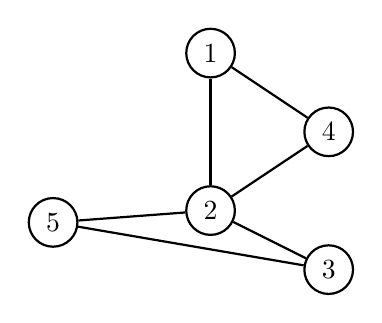
\begin{tikzpicture}
\begin{scope}[every node/.style={circle,thick,draw}]
\node (1) at (0,2) {1};
\node (2) at (0,0) {2};
\node (3) at (1.5,-0.75) {3};
\node (4) at (1.5, 1.) {4};
\node (5) at (-2, -0.15) {5};
\end{scope}
\draw [thick] (1) edge (2);
\draw [thick] (1) edge (4);
\draw [thick] (2) edge (3);
\draw [thick] (2) edge (5);
\draw [thick] (3) edge (5);

\draw [thick] (2) edge (4);

\end{tikzpicture}
\subcaption{Ground truth $A^*$}
\end{minipage}%
\begin{minipage}{0.5\linewidth}
\centering
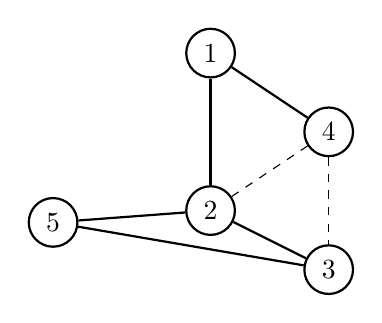
\begin{tikzpicture}
\begin{scope}[every node/.style={circle,thick,draw}]
\node (1) at (0,2) {1};
\node (2) at (0,0) {2};
\node (3) at (1.5,-0.75) {3};
\node (4) at (1.5, 1.) {4};
\node (5) at (-2, -0.15) {5};
\end{scope}
\draw [thick] (1) edge (2);
\draw [thick] (1) edge (4);
\draw [thick] (2) edge (3);
\draw [thick] (2) edge (5);
\draw [thick] (3) edge (5);
\draw [dashed] (2) edge (4);
\draw [dashed] (4) edge (3);
\end{tikzpicture}
\subcaption{Observed graph $A$}
\end{minipage}

\caption{Illustration of the learning problem that we consider. In the left panel, we have the true complete graph $A^*$ which is not observed. The right panel describes our observation: the true edges $(1,2)$, $(1,4)$, $(2,3)$, $(2,5)$, $(3,5)$ are observed, along with the non-existent edges $(1,3)$,$(1,5)$, $(4,5)$ but the information concerning the pairs $(2,4)$ and $(3,4)$ is missing. We aim to decide for $(2,4)$ and $(3,4)$ whether there is a true edge or not.}
\label{lp:fig:setting}
\end{figure}


Let $A^* = (A^*_{i,j})_{1 \leq i,j \leq n}$ be the adjacency matrix of the true complete graph $\cG$, $X \in \R^{n \times d}$ a matrix of node covariates (if available), and $\Omega = (\Omega_{i,j})_{1 \leq i,j \leq n}$ the sampling matrix, such that $\Omega_{i,j} = 1$ if the status (true/false) of $(i,j)$ is observed, and $0$ otherwise. We assume that the entries $\Omega_{ij}$ are i.i.d. random variables and that $\Omega$ is independent from $A^*$ and $X$. 
We denote by $A$ the observed adjacency matrix with $A_{i,j} = \Omega_{i,j} A^*_{i,j}$. Thus, $A_{i,j}=1$ indicates that there is an observed true edge between $i$ and $j$, whereas $A_{i,j}=0$ indicates either the observed lack of an edge or an unreported edge. The sampling matrix $\Omega$ is assumed to be observed, so that it is known which $A_{i,j}=0$ correspond to observed false edges and which correspond to missing information. 
%In addition, we consider that we may have at hand a matrix of node covariates $X \in \R^{n \times d}$.  
The missing information concerns only $A^*$, and not $X$. 
The setting is illustrated in Figure \ref{lp:fig:setting}. 
We denote by $P$ the joint distribution of $Z^* = (A^*, X, \Omega)$, 
%which belongs to a family of distributions $\mathcal{P}$, 
$Z$ the observation $(A, X, \Omega)$ and $\cZ$ the observation space. 

We are interested in classifying the unobserved pairs $\{ (i,j) \; \colon \;  \Omega_{i,j} = 0\}$ into true edges and false edges, based on the observed graph structure. In order to be consistent with the notation of the literature on conformal $p$-values \citep{bates2023testing, liang2022integrative, marandon22b}, we use the following notations:
\begin{itemize}
\item We denote by $\Dtest(Z)=\{ (i,j) \; \colon \;  \Omega_{i,j} = 0\}$ the set of non-sampled pairs and by $\Dtr(Z)=\{ (i,j) \; \colon \;  \Omega_{i,j} = 1\}$ the set of sampled pairs, with $\DtrNull = \{ (i,j) \in \Dtr \; \colon \; A^*_{i,j} = 0 \}$ the set of observed non-existent edges and $\DtrAlt = \{ (i,j) \in \Dtr \; \colon \; A^*_{i,j} = 1 \}$ the set of observed true edges, and we refer to $\Dtest(Z)$ as the test set and to $\Dtr(Z)$ as the training set. 
\item We denote by $\cH_0 = \{(i,j) \; \colon \; \Omega_{i,j} = 0, A^*_{i,j} = 0 \} $ the (unobserved) set of false edges in the test set and $\cH_1 = \{(i,j) \; \colon \; \Omega_{i,j} = 0, A^*_{i,j} = 1 \}$ the (unobserved) set of true edges in the test set. 
\end{itemize}
The notations are summarized in Figure \ref{lp:fig:notations}. 
%with $m_0 = |\cH_0|, \pi_0 = m_0 / m$, with $m_1 = |\cH_1|, \pi_1 = m_1 / m$. 

 %$\Dtest(Z)=\{ (i,j);  \Omega_{i,j} = 0\}$ 
 %$\Dtr(Z)=\{ (i,j);  \Omega_{i,j} = 1\}$
 %$\DtrNull=\{ (i,j);  \Omega_{i,j} = 1, A_{i,j} = 0 \}$
 %$\DtrAlt=\{ (i,j);  \Omega_{i,j} = 1, A_{i,j} = 1 \}$


%We consider the multiple testing problem of controlling the FDR for the null hypothesis
%$$\cH_{0, i,j}\colon A_{i,j} = 0 \quad \text{vs.} \quad \cH_{1, i,j} \colon A_{i,j} = 1 , \quad (i,j) \in \Dtest. $$

\begin{figure}

\begin{minipage}{0.5\linewidth}
\centering
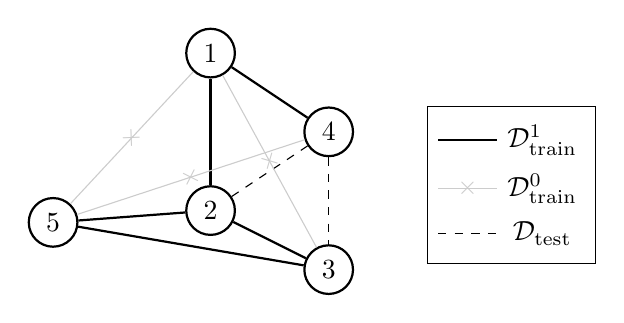
\begin{tikzpicture}
\begin{scope}[every node/.style={circle,thick,draw}]
\node (1) at (0,2) {1};
\node (2) at (0,0) {2};
\node (3) at (1.5,-0.75) {3};
\node (4) at (1.5, 1.) {4};
\node (5) at (-2, -0.15) {5};
\end{scope}
\draw [thick] (1) edge (2);
\draw [thick] (1) edge (4);
\draw [thick] (2) edge (3);
\draw [thick] (2) edge (5);
\draw [thick] (3) edge (5);
\draw [dashed] (2) edge (4);
\draw [dashed] (4) edge (3);
\draw [black!20](1) -- (3) node[pos=0.5, sloped] {\small$\times$}; 
\draw [black!20](4) -- (5) node[pos=0.5, sloped] {\small$\times$}; 
\draw [black!20](1) -- (5) node[pos=0.5, sloped] {\small$\times$}; 

%\draw [red!30!blue!70, bend left] (4) edge (3);
%\draw [red!30!orange!70, bend left] (2) edge (4);


\matrix [draw,xshift=2cm,yshift=-2cm] at (current bounding box.north east) {
  \draw [thick] (0,0) edge (0.75,0); & \node  {$\DtrAlt$}; \\ 
  \draw [black!20] (0,0) -- (0.75,0) node[pos=0.5, sloped] {\small$\times$}; & \node  {$\DtrNull$}; \\
  \draw [dashed] (0,0) edge (0.75,0); & \node  {$\Dtest$}; \\
};
\end{tikzpicture}
%\subcaption{Observed graph $A$}
\end{minipage}
%
\begin{minipage}{0.5\linewidth}
\centering
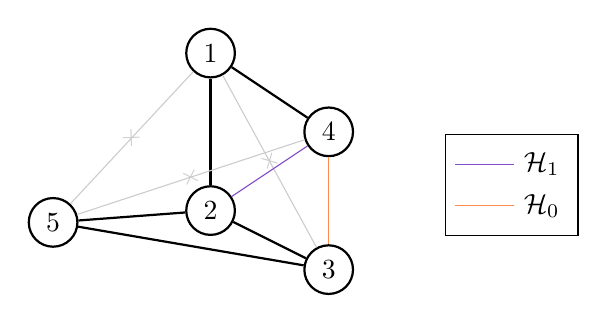
\begin{tikzpicture}
\begin{scope}[every node/.style={circle,thick,draw}]
\node (1) at (0,2) {1};
\node (2) at (0,0) {2};
\node (3) at (1.5,-0.75) {3};
\node (4) at (1.5, 1.) {4};
\node (5) at (-2, -0.15) {5};
\end{scope}
\draw [thick] (1) edge (2);
\draw [thick] (1) edge (4);
\draw [thick] (2) edge (3);
\draw [thick] (2) edge (5);
\draw [thick] (3) edge (5);
\draw [black!20](1) -- (3) node[pos=0.5, sloped] {\small$\times$}; 
\draw [black!20](4) -- (5) node[pos=0.5, sloped] {\small$\times$}; 
\draw [black!20](1) -- (5) node[pos=0.5, sloped] {\small$\times$}; 

\draw [red!30!blue!70] (2) edge (4);
\draw [red!30!orange!70] (3) edge (4);


\matrix [draw,xshift=2cm,yshift=-2cm] at (current bounding box.north east) {
  \draw [red!30!blue!70] (0,0) edge (0.75,0); & \node  {$\cH_1$}; \\
     \draw [red!30!orange!70] (0,0) edge (0.75,0); & \node  {$\cH_0$}; \\ 
};
\end{tikzpicture}
%\subcaption{Observed graph $A$}
\end{minipage}

\caption{Illustration of the notations introduced in Section \ref{lp:sec:meth:not}. The test edges $\Dtest$ (left panel) are divided into two subsets (unobserved): true edges $\cH_1$, and false edges $\cH_0$ (right panel).  } 
\label{lp:fig:notations}
\end{figure}


In our framework, a link prediction procedure is a (measurable) function $R=R(Z)$ that returns a subset of $\Dtest$ corresponding to the indices $(i,j)$ where an edge is declared. 
The aim is to design a procedure $R$ close to $\cH_1$, or equivalently, with $R\cap \cH_0$ (false discoveries) as small as possible. 
For any such procedure $R$, the false discovery rate (FDR) of $R$ is defined as the average of the false discovery proportion (FDP) of $R$ under the model parameter $P\in \mathcal{P}$, 
that is, 
\begin{align*}
\FDR(R)&=\E_{Z^* \sim P} [\FDP(R)],\:\:\: \FDP(R)=\frac{\sum_{i\in \cH_0} \ind_{i\in R}}{1\vee |R|}.%\label{equFDRFDP}
% \E_{Z\sim P}[\FDP(P,R)],\:\:\: \FDP(P,R)=\frac{\sum_{i\in \cH_0} \ind{i\in R}}{1\vee |R|}.\label{equFDRFDP}
\end{align*}
{Similarly, the true discovery rate (TDR) is defined as the average of the true discovery proportion (TDP), that is,}
\begin{align*}
\TDR(R)&= \E_{Z^* \sim P} [\TDP(R)],\:\:\: 
\TDP(R)=\frac{\sum_{i\in \cH_1} \ind_{i\in R}}{1\vee \vert \cH_1 \vert }.%\label{equTDRTDP}
%\TDR(P,R)&= \E_{Z\sim P}[\TDP(P,R)],\:\:\: 
%\TDP(P,R)=\frac{\sum_{i\in \cH_1} \ind{i\in R}}{1\vee m_1(P)}.\label{equTDRTDP}
\end{align*}
Our aim is to build a procedure $R$ that controls the FDR while having a TDR (measuring the \textit{power} of the procedure) as large as possible.


\subsection{Procedure} \label{lp:sec:meth:def}

%In this section, we describe the procedure. 

It is assumed that we have at hand a \textit{link prediction} function $g: V \times V \times  \cZ \rightarrow \R$ (henceforth called \textit{scoring} function), which takes as input a pair $(i,j)$ and an observation $z \in \cZ$ %(i.e. $z=(a,x,\omega)$ with graph $a \in \R^{n \times n}$, a matrix of covariates $x \in \R^{n \times d}$, and a sampling matrix $\omega \in \R^{n \times n}$),
and returns a \textit{score} $S_{i,j} \in \R$, estimating how likely it is that $i$ is connected to $j$. The score does not have to be in $[0,1]$: for instance, $S_{i,j}$ can be the number of common neighbors between $i$ and $j$. %Most often, it does denote a probability, such as is returned by supervised learning approaches like SEAL/VGAE/SBM etc. 


%In any case, such output only gives a ranking of the pairs, from most likely to least likely to be a true edge. In particular, considering the case where scores denote probabilities, declaring as edges the pairs $(i,j) \in \Dtest$ for which their score $S_{i,j}$ is above $0.5$, or $1-\alpha$, will not lead in general to a set of edges such that the FDR is below $\alpha$ (as shown in the numerical experiments, see Section \ref{sec:numexp}). 

To obtain a set of edges with FDR below $\alpha$, we borrow from the literature on knockoffs and conformal inference \citep{weinstein2017power, bates2023testing} to formulate the following idea: some of the observed false edges can be used as a reference set, % to estimate the FDP that would occur for a cut-off $t$. 
by comparing the score for a pair in the test set to scores computed on false edges to determine if it is likely to be a false positive. 
%\textit{significantly} high. 
%
Effectively, we will declare as edges the pairs that have a test score higher than a cut-off $\hat t$ computed from the reference set and depending on the level $\alpha$. In detail, the steps are as follows:
\begin{enumerate}
\item Build a set of false edges by sampling uniformly from $\DtrNull$. We call this set $\Dcal$ and we refer to it as a \textit{reference set};%, or a calibration set;

\item Learn a scoring function $g$ (whose specific form will be given later) and compute the scores for the reference set and for the test set;%$S_{i,j}$ for $(i,j) \in \Dcal \cup \Dtest$. 

\item Declare as true edges the pairs in the test set that are returned by the Counting Knockoff (CK) algorithm \citep{weinstein2017power} given in Algorithm \ref{lp:algo:CK}. 
\end{enumerate}
The CK algorithm \citep{weinstein2017power} comes from the knockoffs literature and is equivalent to the conformal $p$-value procedure of \cite{bates2023testing} (see \citealp{mary2022semi}). 
It is a stepwise procedure which looks for the appropriate cut-off $\hat t$ among a suitable range of values $\cT$ by using the reference scores as benchmarks to evaluate how many false discoveries there are among the selected set of test edges for any cut-off $t \in \cT$. The CK algorithm is illustrated in Figure \ref{lp:fig:CK}.

\begin{algorithm}[t]
Input: {test scores $(S_w)_{w \in \Dtest}$, knockoff scores $(S_w)_{w \in \Dcal}$.}\\
1. Order the scores from lowest to highest, that is $S_{(1)} \geq S_{(2)} \geq \dots \geq S_{( \vert \Dcal \vert + \vert \Dtest \vert)}$\\
2. Let $s_\ell$ be the label of $S_{(\ell)}$ \\
3. Set $\FDP=1$, $V=\vert \Dcal \vert$, $\ell=\vert \Dcal \vert + \vert \Dtest \vert$, $K=\vert \Dtest \vert$ \\
4. While $\widehat \FDP \leq \alpha$ and $K\geq 1$ do $\ell=\ell-1$
\begin{itemize}
\item if $s_{\ell+1} = 1$, $V=V-1$
\item else, $K=K-1$
\item do $\FDP= \frac{V+1}{\vert \Dcal \vert+1} \frac {\vert \Dtest \vert}{K}$ (or $\FDP = 1$ if $K=0$) 
\end{itemize}
Output: { $\{w \in \Dtest \colon S_w \geq S_{(K)} \}$ (return the empty set if $K=0$).}
  \caption{Counting Knockoff \citep{weinstein2017power}}\label{lp:algo:CK}
\end{algorithm}


\begin{figure}
\centering

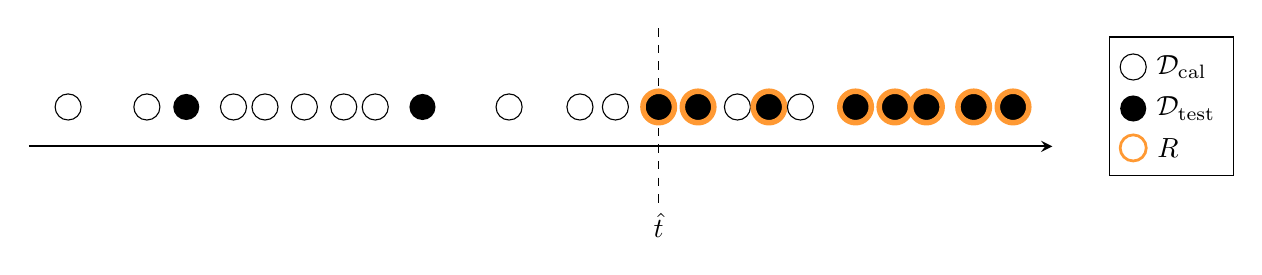
\begin{tikzpicture}[nullnode/.style={circle, draw},%minimum size
testnode/.style={circle, fill=black},
rejnode/.style={circle, draw=orange!80, line width= 2pt, fill=black, minimum size=4mm}, ]

\draw [thick, ->, >=stealth] (-5,0) -- (8,0);


\node [nullnode] at (-4.5,0.5) {};
\node [nullnode] at (-3.5,0.5) {};
\node [testnode] at (-3,0.5) {};
\node [nullnode] at (-2,0.5) {};
\node [nullnode] at (-2.4,0.5) {};
\node [nullnode] at (-1.5,0.5) {};
\node [nullnode] at (-1.,0.5) {};
\node [nullnode] at (-0.6,0.5) {};
\node [testnode] at (0,0.5) {};
\node [nullnode] at (1.1,0.5) {};
\node [nullnode] at (2.,0.5) {};
\node [nullnode] at (2.45,0.5) {};
\node [rejnode] at (3,0.5) {};
\node [rejnode] at (3.5,0.5) {};
\node [nullnode] at (4,0.5) {};
\node [rejnode] at (4.4,0.5) {};
\node [nullnode] at (4.8,0.5) {};
\node [rejnode] at (5.5,0.5) {};
\node [rejnode] at (6,0.5) {};
\node [rejnode] at (6.4,0.5) {};
\node [rejnode] at (7,0.5) {};
\node [rejnode] at (7.5,0.5) {};

\node (t) at (3, -1) {$\hat t$}; 
\draw [dashed] (3, 1.5) -- (t); 


\matrix [draw,xshift=1.5cm,yshift=-1cm] at (current bounding box.north east) {
  \node [nullnode, label=right:$\Dcal$] {}; \\
   \node [testnode, label=right:$\Dtest$] {} ;\\
    \node [circle, draw=orange!80, line width= 1pt, label=right:$R$] {};\\
};

\end{tikzpicture}
\caption{Illustration of the CK algorithm (Algorithm \ref{lp:algo:CK}). The procedure looks for the cut-off $\hat t$ by going from the smallest values of the scores% test statistics 
 (left) to the largest values (right), and stops as soon as the FDP falls below $\alpha$. At each step, the FDP is estimated by the proportion of reference scores among the scores in the left part.
} \label{lp:fig:CK}
\end{figure}


The full procedure is given in Algorithm \ref{lp:algo:main} and is illustrated in Figure \ref{lp:fig:proc}. 
We next describe our proposal for choosing the scoring function $g$.

\begin{algorithm}[t]
Input: {Adjacency matrix $A$, node covariates matrix $X$, sampling matrix $\Omega$, link prediction function $g$, reference set sample size}\\
1. Sample $\Dcal$ uniformly from $\DtrNull$ \\
%If $\Omega_{i,j} | A, X \overset{i.i.d.}{\sim} U_{V \times V}$: Sample $\Dcal$ uniformely from $\DtrNull$ \\
 %Otherwise: 
 	%\begin{itemize}
 	%\item Sample $\tilde \Omega$ as described in Section \ref{sec:refset}
	%\item Set $\Dcal = \{ (i,j), \tilde \Omega_{i,j} = 0 \} \cap \DtrNull$
	%\item Do $A \leftarrow \tilde \Omega \odot A$, $\Dtr  \leftarrow \Dtr \backslash ( \{ (i,j), \tilde \Omega_{i,j} = 0 \} \cap \DtrAlt) $,  $\Omega \leftarrow \tilde \Omega$ 
	%\end{itemize}
2. Learn $g$ on $Z=(A, X, \Omega)$, of the form \eqref{lp:eq:scorefn2} \\
3. For each $(i,j) \in \Dcal \cup \Dtest$, compute the score $S_{i,j} = g((i,j), Z)$ \\
4. Apply Algorithm \ref{lp:algo:CK} using as input $(S_{i,j})_{(i,j) \in \Dtest}$ for the test scores and $(S_{i,j})_{(i,j) \in \Dcal}$ for the reference scores \\
Output: { R(Z) = set $\subset \Dtest$ returned in previous step.} %$\{w \in \Dtest \colon S_w \geq S_{(K)} \}$ (return the empty set if $K=0$).}
  \caption{Conformal link prediction}\label{lp:algo:main}
\end{algorithm}

\begin{remark} This type of procedure is designed to control the FDR at level $\frac{ \vert \cH_0 \vert} {\vert \Dtest \vert} \alpha < \alpha$. To maximize power, we recommend to apply the procedure at level $\alpha / \hat \pi_0$ where $\hat \pi_0 \in ]0,1[$ is an estimate of $\frac{ \vert \cH_0 \vert} {\vert \Dtest \vert}$. In our setting, it is assumed that $\Omega$ is independent of $A^*$, so $\hat \pi_0 = \frac{ \vert \DtrNull \vert} {\vert \Dtr\vert}$ is expected to be a reliable estimate. Alternatively, tools from the multiple testing literature on the estimation of the proportion of null hypotheses may be employed, e.g. by using Storey's estimator \citep{marandon22b}. 
\end{remark}



\subsection{Choice of the scoring function $g$}  \label{lp:sec:meth:score}

There are two desiredata concerning the choice of the scoring function $g$: 
\begin{itemize}
\item [(i)] A key point is that the reference scores mimic the scores $(S_{i,j})_{i,j \in \cH_0}$ of the false edges in the test set in such a way that, if $(i,j) \in \cH_0$ then
the rank of $S_{i,j}$ among the reference scores should be uniformly distributed, allowing good estimation of the FDP in the CK algorithm. 
This property is properly formalized and discussed in Appendix  \ref{lp:app:exch}.
Here, it entails that the scoring function $g$ must be chosen carefully, because of the dependence structure in the data. 
\item [(ii)]To fulfill the above property, it is not needed that the quality of the estimates $S_{i,j}$ be particularly good. However, to maximize power, it is desirable that the scores are as close as possible to the true probabilities $\P( A^*_{i,j}=1 \; \vert \; Z)$ up to a strictly monotone transformation. %In particular, \textit{learning} $g$ from the data is expected to offer the most power. 
\end{itemize}



To address the afore-mentioned points, the scoring function $g$ will be taken as the output of a link prediction technique of choice, that will be learned with a suitable modification of the input. 
Define a link prediction algorithm $\hat P \colon (i,j) \in V \times V, z \in \cZ \mapsto \hat P_{i,j} (z)$, where $\hat P_{i,j}$ is the prediction for the pair $(i,j)$ given the observation $z$. In a nutshell, given a link prediction algorithm $\hat P$, the scoring function $g (\cdot, Z) $ is taken as 
$\hat P( \cdot, \tilde Z)$, where $\tilde Z$ is obtained from $Z$ by setting to zero the entries of the sampling matrix that correspond to the reference set $\Dcal$:
\begin{align} \label{lp:eq:inputmodif}
\tilde Z = (A, X, \tilde \Omega), \quad \tilde \Omega_{i,j}= \begin{cases}
      0, & \text{if}\ (i,j) \in \Dcal  \\
      \Omega_{i,j}, & \text{otherwise.}
    \end{cases}
\end{align}
In words, taking $g(\cdot,Z) = \hat P( \cdot, \tilde Z) \neq \hat P(\cdot, Z)$  amounts to learn the link predictor by treating the edge examples in the reference set as non-observed pairs in the algorithm.
We elaborate on this later, after formalizing explicitly the output of LP methods.
%We start by formalizing explicitly the output of link prediction techniques. Then, we detail how to build a suitable score using such a link prediction technique of choice.

\paragraph{Link prediction}% in practice: formalization of the output} 

For simplicity of presentation, let us consider here an undirected graph with no node covariates. Let us introduce, for a given $K \in \{1, \dots, n \}$ the r.v.
\begin{align} \label{lp:eq:Khop}
W_{i,j} = (A_{i, \bullet}, A_{j, \bullet}, A^2_{i, \bullet}, A^2_{j, \bullet}, \dots, A^K_{i, \bullet}, A^K_{j, \bullet}), 
\end{align}
where $A^k_{i, \bullet} = (A^k_{i, u})_{1\leq u \leq n}$ for $1 \leq k \leq K$.
The r.v. \eqref{lp:eq:Khop} can be thought of as the "$K$-hop neighborhood" of $(i,j)$. It represents a type of embedding for the pair $(i,j)$, that describes a \textit{pattern} of connection around $i$ and $j$. If the graph displays structure, then it should be observed that the motif of the pattern differs when $i$ and $j$ are connected compared to when they are not. Moreover, there should be some similarity between the patterns observed for true edges, as compared to false edges. Figure \ref{lp:fig:embedding} gives an illustration in the case of a graph with community structure. When there is an edge between $i$ and $j$ (Figure \ref{lp:fig:embeddingtrue}), $i$ and $j$ are both involved in a same group of nodes that is densely connected (community). Conversely, when there is no edge between them (Figure \ref{lp:fig:embeddingfalse}), $i$ and $j$ are involved in separate groups of densely connected nodes that share few links between them. 

\begin{figure}

\begin{minipage}{0.5\linewidth}
\centering
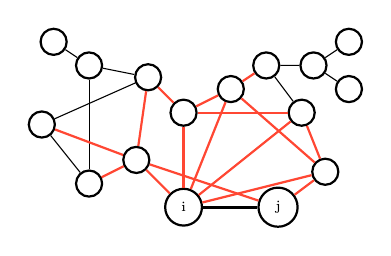
\begin{tikzpicture}[scale=0.6, every node/.style={scale=0.6}]

\tikzstyle{hop} = [thick,red!80!orange!80]


\begin{scope}[every node/.style={circle,thick,draw}]
\node [minimum size=4mm] (i) at (0,0) {\tiny i};
\node [minimum size=4mm] (j) at (2,0) {\tiny j};

\node (1) at (-1,1) {};
\node (2) at (-0.75,2.75) {};
\node (3) at (0,2) {};
\node (4) at (1,2.5) {};
\node (5) at (3,0.75) {};
\node (6) at (2.5,2) {};

\node (7) at (-2,0.5) {};
\node (8) at (-2,3) {};
\node (9) at (-2.75,3.5) {};
\node (10) at (-3,1.75) {};
%\node (11) at (-3,0) {};
\node (12) at (1.75,3) {};
\node (13) at (2.75,3) {};
\node (14) at (3.5,3.5) {};
\node (15) at (3.5,2.5) {};

\end{scope}

\draw [very thick] (i) edge (j);

\draw [hop] (1) edge (i);
\draw [hop] (1) edge (j);
%\draw (2) edge (i);
%\draw (2) edge (j);
\draw [hop]  (3) edge (i);
%\draw [hop] (3) edge (j);
\draw [hop] (4) edge (i);
%\draw (4) edge (j);
\draw [hop] (5) edge (i);
\draw [hop] (5) edge (j);
\draw [hop] (6) edge (i);
%\draw [hop] (6) edge (j);

\draw [hop] (1) edge (2);
\draw [hop] (2) edge (3);
\draw [hop] (3) edge (4);
\draw [hop] (4) edge (5);
\draw [hop] (5) edge (6);
\draw [hop] (3) edge (6);
\draw [hop] (7) edge (1);
\draw (8) edge (2);
\draw (9) edge (8);
\draw (10) edge (7);
%\draw (11) edge (7);
\draw [hop] (4) edge (12);
\draw (6) edge (12);
\draw (12) edge (13);
\draw (10) edge (2);
\draw (8) edge (7);
\draw (13) edge (14);
\draw (13) edge (15);
\draw [hop]  (1) edge (10);


\end{tikzpicture}
\subcaption{True edge} \label{lp:fig:embeddingtrue}
\end{minipage}%
\begin{minipage}{0.5\linewidth}
\centering
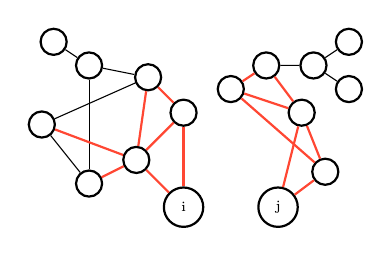
\begin{tikzpicture}[scale=0.6, every node/.style={scale=0.6}]

\tikzstyle{hop} = [thick,red!80!orange!80]

\begin{scope}[every node/.style={circle,thick,draw}]
\node [minimum size=5mm] (i) at (0,0) {\tiny i};
\node [minimum size=5mm] (j) at (2,0) {\tiny j};

\node (1) at (-1,1) {};
\node (2) at (-0.75,2.75) {};
\node (3) at (0,2) {};
\node (4) at (1,2.5) {};
\node (5) at (3,0.75) {};
\node (6) at (2.5,2) {};
\node (7) at (-2,0.5) {};
\node (8) at (-2,3) {};
\node (9) at (-2.75,3.5) {};
\node (10) at (-3,1.75) {};
%\node (11) at (-3,0) {};
\node (12) at (1.75,3) {};
\node (13) at (2.75,3) {};
\node (14) at (3.5,3.5) {};
\node (15) at (3.5,2.5) {};

\end{scope}

\draw [hop] (1) edge (i);
\draw [hop] (1) edge (2);
\draw [hop] (1) edge (3);
%\draw (2) edge (i);
\draw [hop] (2) edge (3);
\draw [hop] (3) edge (i);

%\draw (4) edge (j);
\draw [hop] (4) edge (5);
\draw [hop] (4) edge (6);
\draw [hop] (5) edge (j);
\draw [hop] (5) edge (6);
\draw [hop] (6) edge (j);

\draw [hop] (7) edge (1);
\draw (8) edge (2);
\draw (9) edge (8);
\draw (10) edge (7);
%\draw (11) edge (7);
\draw [hop] (4) edge (12);
\draw [hop] (6) edge (12);
\draw (12) edge (13);
\draw (10) edge (2);
\draw (8) edge (7);
\draw (13) edge (14);
\draw (13) edge (15);
\draw [hop]  (1) edge (10);

\end{tikzpicture}
\subcaption{False edge} \label{lp:fig:embeddingfalse}
\end{minipage}

\caption{Example of K-hop (K=2) neighborhood of $(i,j)$ (in color), for when (a) $i$ and $j$ are connected and (b) $i$ and $j$ are not connected. }
\label{lp:fig:embedding}
\end{figure}

Link prediction methods output a prediction $\hat P_{i,j} \in \R$, indicating the relevance of an edge between $i$ and $j$. In general, the prediction can be written as 
\begin{align} \label{lp:eq:scorelp}
 \hat P_{i,j}(Z) = h( W_{i,j}; \{(W_{u,v}, A_{u,v}), (u,v) \in \Dtr \}), 
\end{align}
with $h$ some real-valued measurable function. In \eqref{lp:eq:scorelp}, the set $\{(W_{u,v}, A_{u,v}), (u,v) \in \Dtr \}$ represents a set of learning examples, where $W_{u,v}$ is an embedding for the pair $(u,v)$ and $A_{u,v}$ is its label.
For instance, in the case of the common neighbors (CN) heuristic, the number of common neighbors is given by the scalar product $A_{i, \bullet}^T A_{j, \bullet}$. In that case, the prediction is $\hat P_{i,j}  = h( W_{i,j}) = A_{i, \bullet}^T A_{j, \bullet}$. 
Alternatively, when considering supervised approaches such as binary classification \citep{zhang2018link, bleakley07}, maximum likelihood  \citep{kipf2016variational, chiquet20} or matrix completion \citep{levina23, gaucher21}, the link prediction function can be written as the minimizer of an empirical risk (ERM): 
\begin{align} \label{lp:eq:scoreERM}
&\hat P_{i,j}(Z) = \hat h (W_{i,j}), \\ 
&\hat h \in  \underset{h \in \cF}{\argmin} \sum_{(i,j) \in \cD} \cL[ P_{i,j}, A_{i,j} ], \quad P_{i,j} = h(W_{i,j}) 
\end{align}
with $\cL : [0,1] \times \{0,1\} \rightarrow \R$ a loss function, $\cF$ a function class, and $\cD$ a certain subset of $\Dtr$. In \eqref{lp:eq:scoreERM}, $P_{i,j} $ is an estimate of the probability that there is an edge between $i$ and $j$, and the error term $\cL[ P_{i,j}, A_{i,j} ]$ quantifies the difference between the prediction $P_{i,j}$ and the truth $A_{i,j} $. %In \eqref{eq:scorefnERM}, $f((i,j), Z)$ represents the prediction for $(i,j)$ i.e. the estimated probability that there is an edge between $i$ and $j$. 
The ERM formulation for the supervised approaches afore-mentioned can be justified as follows: 
	\begin{itemize}
		\item Binary classification approaches \citep{zhang2018link, bleakley07}: In that case the ERM formulation \eqref{lp:eq:scoreERM} is obvious. For instance, for SEAL \citep{zhang2018link}, $P_{i,j}$  is given by a GNN that takes as input the $K$-hop subgraph around $(i,j)$, excluding the edge between $(i,j)$ if there is one observed, and augmented with node features that describe the distance of each node to $i$ and to $j$. The parameters of the GNN are fitted by minimizing the cross-entropy loss over a set $\cD \subset \Dtr$ of observed true/false edges. In practice, $\cD$ is subsampled from $\Dtr$ in order to have a $50\%-50\%$ repartition between true edges and false edges. %usually
				
	\item Maximum likelihood approaches \citep{kipf2016variational, chiquet20}: Maximum likelihood approaches aim to optimize a lower bound on the likelihood (ELBO). This lower bound is an expectation and therefore, using Monte-Carlo approximation, we end up with a function of the form \eqref{lp:eq:scoreERM}. For instance, for VGAE \citep{kipf2016variational}, $P_{i,j}$ is given by the scalar product $H_i^T H_j$ where $H_u$ is a \textit{node embedding} for node $u$, the embedding matrix $H \in \R^{n \times n}$ being the output of a GNN. It follows that $H_u = h(A_{u, \bullet},  A^2_{u, \bullet}, \dots, A^L_{u, \bullet})$ for some function $h$, with $L$ the number of layers of the GNN. 

	\item Matrix completion \citep{levina23, gaucher21}: e.g., for \cite{levina23}, one can rewrite the estimated probability matrix $\hat P$ as $\hat P =  \argmin_{P} \{ \sum_{(u,v) \in \Dtr} (A_{u,v} - P_{u,v})^2, P = A_{in}^T\Theta A_{in}, \; \text{rank}(\Theta) \leq r\}$ where $A_{in}$ is the sub-matrix of $A$ consisting only of the observed entries. Hence, in that case, $\hat P_{i,j}$ is of the form \eqref{lp:eq:scoreERM} with $P_{i,j}=h(A_{i, \bullet}, A_{j, \bullet})$ for some function $h$. 
	\end{itemize}


\paragraph{Construction of the scoring function $g$} Given a link prediction algorithm $\hat P$, the scoring function $g$ is given by
\begin{align} \label{lp:eq:scorefn1}
g((i,j), Z) = \hat P((i,j), \tilde Z), %= \hat P_{i,j}( \tilde Z)
\end{align}
with $\tilde Z$ previously defined in \eqref{lp:eq:inputmodif}. The input $\tilde Z = (A, X, \tilde \Omega)$ to the LP algorithm $\hat P$ consists of a modification of $Z$, which enforces that the edge examples $(i,j)$ in the reference set $\Dcal$ are treated as unreported information (i.e., the same as $\Dtest$) by the algorithm.
To put it differently, given equation \eqref{lp:eq:scorelp}, the scoring function $g$ is then of the form
\begin{align} \label{lp:eq:scorefn2}
g((i,j), Z) &= h( W_{i,j}; \{(W_{u,v}, A_{u,v}), (u,v) \in \Dtr \backslash \Dcal \}) 
\end{align}
with $h$ some real-valued measurable function. 


Treating the reference set $\Dcal$ as unreported information when learning the score in \eqref{lp:eq:scorefn1}, or equivalently, removing $\Dcal$ from the set of learning examples in \eqref{lp:eq:scorefn2}, is necessary to fabricate good reference scores and avoid biasing the comparison of the test scores to the reference scores in the CK Algorithm. Otherwise, the scoring $g$ may use the knowledge that the pairs in the reference set are false edges and produce an overfitted score for those. 

%\subsubsection{Choice of the reference set $\Dcal$}  \label{sec:refset}
%Given the choice of $g$ layed out in the previous paragraph, to fabricate reference scores ensuring FDR control in Algorithm \ref{algo:CK} one would like the $K$-hop neighborhood of any negative edge in the test set to be \textit{approximately exchangeable}  (see Assumption \ref{ass:exch}) with the $K$-hop neighborhood of the negative edges in the reference set $\Dcal$. 
%However, this won't necessarily be the case if we select $\Dcal$ in a completely random manner. To see this, consider that $\Dtest$ is actually sampled by sampling some proportion of the nodes, say 5\%, and removing some fixed proportion of their positive and negative edges, say 50\% for each. This particular type of missing data pattern is called egocentric sampling \citep{levina23} and is typical of data collected from surveys. In that situation, neighborhoods of missing negative edges will look \textit{depleted} compared to neighborhoods of observed negative edges. 
%In particular, Assumption  \ref{ass:exch} will be very much violated, and in general the FDR will not be controlled at level $\alpha$. 

%To remedy this issue we propose the following. Let $P_{\Omega \vert A^*, X}$ be the conditional distribution of $\Omega$ given $(A^*, X)$. Let us assume that it is known, and that it is not completely uniform i.e. missing edges are not sampled uniformly from $V \times V$ (otherwise, there is no issue and we just sample $\Dcal$ uniformly from $\DtrNull$). We propose to sub-sample the observed graph $A$ according to some \textit{scaling} of $P_{\Omega \vert A^*, X}$: that is, given a fixed number $\vert \Dcal \vert$ of negative edges to remove (i.e. label as missing), we would like to sub-sample from $\Dtr$ in such way that the sampling matrix $\tilde \Omega$ has its \textit{local structure} similar to that of samples from $P_{\Omega \vert A^*, X}$. 

%To explain concretely what we mean, let us go back to the example of egocentric sampling where $\Omega$ is sampled by removing 50\% of both positive and negative edges for 5\% of the nodes. In that case our proposal translates to sampling $\tilde \Omega$ by removing 50\% of the positive and negative edges from a proportion $p$ of nodes, where $p$ is computed so that the constraint $\sum_{i,j \in \DtrNull} \tilde \Omega_{i,j} =  \vert \Dcal \vert$ is satisfied. It is seen that, compared to $P_{\Omega \vert A^*, X}$, the proportion of nodes for which we remove edges is adjusted while the proportion of edges removed per node is kept the same. That way, neighborhoods of the negative edges $(i,j)$ for which $\tilde \Omega_{i,j}=0$ will be \textit{similarly depleted} compared to those of the missing negative edges $\cH_0$. 
%$\tilde \Omega_{i,j} = 1$ if $(i,j) \in \Dtr \backslash \Dcal$ and $0$ otherwise 

%Afterwards, the negative edges $(i,j)$ such that $\tilde \Omega_{i,j}=0$ are put in $\Dcal$. Importantly, the sampled positive edges are also effectively removed from the training set learning samples. To keep consistent with the notation in the formulation \eqref{eq:scorefnERM}, this entails that $\Dtr$ and $A$ in \eqref{eq:scorefnERM} become, $\Dtr \backslash ( \{ (i,j), \tilde \Omega_{i,j} = 0 \} \cap \DtrAlt) $ and $ \tilde \Omega \odot A$, respectively. %$g$ will be learned on the observation $(\tilde A, \tilde \Omega, X)$ where $\tilde A = \tilde \Omega \odot A$. 



%in practice, we don"t know the exact parameters, but we may have an intuition of how it works depending on the context. [give examples] in any case, at least on principle, if MCAR, it can be deduced/learned from $\Omega$. otherwise, ...outside of the scope here / leave this to future research. 






We outline a key property of our method when $g$ is learned with a binary classification approach, which includes state-of-the-art LP methods, such as \cite{zhang2018link}. In practice, in this type of approach, for an observation $z$, the set $\cD(z)$ of learning examples in \eqref{lp:eq:scoreERM} is chosen to be a strict subset of $\Dtr(z)$ with a $50\%-50\%$ repartition between true edges and false edges. 
Since real-world networks are sparse, $\cD(z)$ then consists of the observed true edges $\DtrAlt(z)$ and a sub-sample of the observed false edges $\DtrNull(z)$ in the same amount.
Now, learning the scoring function $g$ as previously described requires to have no overlap between the reference set $\Dcal$ and the set of learning examples: this is enforced by learning the link predictor with the input $\tilde Z$, so that the set of learning examples is $\cD(\tilde Z) \subset \Dtr(\tilde Z)$, and $\cD (\tilde Z) \cap \Dcal = \emptyset$. Then, a concern is that we have $\cD(\tilde Z) \subset \cD(Z)$: the "input modification" that consists of using $\tilde Z$ instead of $Z$ effectively reduces the size of the set of learning examples that the score is learned with, which could lead to power loss as compared to a method that utilizes $Z$ directly. 
However, since there is large number of false edges that are discarded in the first place when building $\cD(z)$ for any observation $z$, the reference set $\Dcal$ can be selected so that $\cD(\tilde Z) = \cD(Z)$ is actually true. Therefore, the amount of learning examples is the same before and after the input modification. Thus, the input modification is free of any trade-off regarding the quality of $g$. 


\begin{figure}
\centering
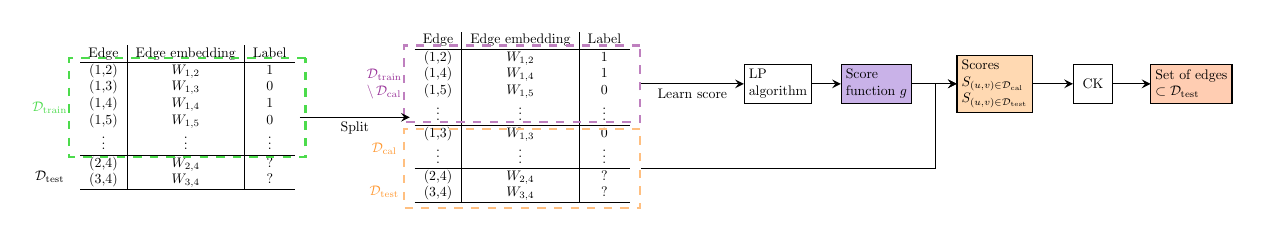
\begin{tikzpicture}[node distance = 3.5cm, scale=0.5, every node/.style={transform shape}]

\tikzstyle{box} = [rectangle, minimum width=6cm, minimum height=2.5cm, dashed]
\tikzstyle{box2} = [rectangle, minimum width=1cm, minimum height=1cm, draw=black]
\tikzstyle{arrow} = [->,>=stealth]


\node (data) at (0,0){
\begin{tabular}{c|c|c}
Edge & Edge embedding & Label \\ %add "Edge/pair"? 
\hline
(1,2) & $W_{1,2}$ & 1 \\
(1,3) & $W_{1,3}$ & 0 \\
(1,4) & $W_{1,4}$ & 1 \\
(1,5) & $W_{1,5}$ & 0 \\
$\vdots$ & $\vdots$ & $\vdots$ \\
\hline
(2,4) & $W_{2, 4}$ & ? \\
(3,4) & $W_{3, 4}$ & ? \\
\hline
\end{tabular}
}; 
\node (dtrain) [left of=data, yshift=2.5mm, text=green!80!black!70] {$\Dtr$};
\node (dtest)  [left of=data, yshift=-1.5cm]{$\Dtest$};
\node (dtrainbox) [box, right of=dtrain, draw=green!80!black!70, thick] {}; 
\node (dtestbox) [box, right of=dtest, minimum height=0.80cm] {}; 

\node (newdata)[right of=data, xshift=5cm]{
\begin{tabular}{c|c|c}
Edge & Edge embedding & Label \\ %add "Edge/pair"? 
\hline
(1,2) & $W_{1,2}$ & 1 \\
(1,4) & $W_{1,4}$ & 1 \\
(1,5) & $W_{1,5}$ & 0 \\
$\vdots$ & $\vdots$ & $\vdots$ \\
\hline
(1,3) & $W_{1,3}$ & 0 \\
$\vdots$ & $\vdots$ & $\vdots$ \\
\hline
(2,4) & $W_{2, 4}$ & ? \\
(3,4) & $W_{3, 4}$ & ? \\
\hline
\end{tabular}
}; 
\node (dtrain2) [left of=newdata, yshift=0.85cm, align=left, text=red!50!blue!80] {$\Dtr$ \\ $\backslash \Dcal$};
\node (dtest2)  [left of=newdata, yshift=-1.9cm, text=orange!80]{$\Dtest$};
\node (dcal)  [left of=newdata, yshift=-0.8cm, text=orange!80]{$\Dcal$};
\node (dtrainbox2) [box, right of=dtrain2, minimum height=1.95cm, draw=red!50!blue!50, thick] {}; 
\node (dtestbox2) [box, right of=dtest2, minimum height=0.80cm] {}; 
\node (dcalbox) [box, right of=dcal, minimum height=1cm] {}; 
\node (dtestcalbox) [box, right of=dcal, minimum height=2cm, draw=orange!50, thick, yshift=-0.5cm] {}; 

\node (algo) [box2, right of=dtrainbox2, xshift=3cm, align=left] {LP \\ algorithm}; 
\node (score) [box2, right of=algo, align=left, xshift=-1cm, fill=red!30!blue!30] { Score \\ function $g$}; 
\node(mid)[right of=score, xshift=-2cm] {};
\node (compute) [box2, right of=mid, align=left, fill=orange!30, xshift=-2cm] {Scores \\ $S_{(u,v) \in \Dcal}$ \\$ S_{(u,v) \in \Dtest}$}; 
\node (CK) [box2, right of=compute, xshift=-1cm] {CK}; 
\node (out) [box2, right of=CK, align=left, xshift=-1cm, fill=red!30!orange!30] {Set of edges \\ $\subset \Dtest$}; 



\draw [arrow] (data)--(newdata) node[midway, below]{Split}; 
\draw [arrow] (dtrainbox2)--(algo) node[midway, below]{Learn score}; 
\draw [arrow] (algo)--(score); 
\draw  (score)--(mid); 
\draw  [arrow] (mid)--(compute); 
%\draw (score)--(compute); 
\draw [arrow] (score)--(compute); 
%\draw [arrow] ([yshift=0.5cm] dtestbox2)-|(compute); 
\draw (dtestcalbox)-|( [yshift=0.15cm] mid.south); 
\draw [arrow] (compute)--(CK); 
\draw [arrow] (CK)--(out); 

%\draw [decorate,
    %decoration = {brace}, yshift=-1cm] (data.west) --  (data.north west);
    
\end{tikzpicture}
\caption{Illustration of the procedure proposed in this work.} \label{lp:fig:proc}
\end{figure}



\section{Numerical experiments} \label{lp:sec:numexp}

In this section, we study the performance of our method both on simulated data (Section \ref{lp:sec:simu}) and real data (Section \ref{lp:sec:realdata}). We consider two choices for the scoring function $g$, SEAL \citep{zhang2018link}  (see Appendix \ref{lp:app:expdetails} for details) and CN, which gives the procedures \texttt{CN-conf} and \texttt{SEAL-conf}. 
We compare the performance of our method to two "naive" procedures for FDR control (here we assume that $g \in [0,1]$, otherwise, scores are normalized into $[0,1]$ by standardizing the values and applying the sigmoid function): %i.e. g((i,j), Z) estimates the prob. 
\begin{itemize}
\item \textit{Naive thresholding} (NT): We select into $R(Z)$ the edges $(i,j) \in \Dtest$ for which $ g((i,j), Z) \geq 1-\alpha$. %, that is $R(Z) = \{ g((i,j), Z) \geq 1- \alpha, (i,j) \in \Dtest \}$. 
If the probabilities $g((i,j), Z)$ are poorly estimated, this procedure is expected to not control the FDR at level $\alpha$ in general.
\item \textit{Cross-validated thresholding} (CVT): We set aside a validation sample $\Dval \subset \Dtr$ and learn $g$ on the remaining data, then compute from a range of values $T \subset [0,1]$  the maximum threshold $\hat t \in T$ for which the FDP on $\Dval$ is below $\alpha$. Then we select into $R(Z)$ the edges $(i,j) \in \Dtest$ for which $ g((i,j), Z) \geq \hat t$. To start with, this procedure is not very convenient because it needs to be fed a range of cut-offs values T, which specification is not obvious. Moreover, it is expected to perform fine only if the validation set is large enough, otherwise it will fail. For small $n$, this is a clear disadvantage compared to our method: ours requires only non-existent edges examples, which are always largely available due to real-world networks being sparse, and the full set of observed true edges is utilized for training. Here, we set $\vert \Dval \vert$ to $20\% \vert E \vert$ with a 50\%-50\% repartition between true edges and non-existent edges, and $T = \{ (1-\alpha)/k, k \in \{1, 5, 10, 20, 50, 100 \} \} $.

\end{itemize}

%We apply our procedure, and the baselines, with two choices for the scoring function $g$, SEAL \citep{zhang2018link} and the Common Neighbors (CN) heuristic, which gives the procedures \texttt{CN-conf}, \texttt{SEAL-conf},  \texttt{CN-NT},   \texttt{SEAL-NT},  \texttt{CN-CVT}, \texttt{CN-CVT}. 


 In each experiment, the FDR and TDR of the different methods are evaluated by using 100 Monte-Carlo replications. 

\subsection{Simulated data} \label{lp:sec:simu}
In this section, we evaluate our method on a simulated dataset. 
We generate a graph $A^*$ of $n=100$ nodes from a Stochastic Block Model (SBM) with $5$ classes, mixture proportions $\pi = (1/5, \dots 1/5)$, and connectivity matrix $\gamma$ given by
\begin{align*}
\gamma = 
\begin{pmatrix}
\epsilon &p &p &p & \epsilon \\
p & \epsilon & p & \epsilon & \epsilon \\
p &p &p &\epsilon & \epsilon \\
p &\epsilon &\epsilon &\epsilon &\epsilon \\
\epsilon &\epsilon &\epsilon &\epsilon &p 
\end{pmatrix}, 
\end{align*}
with $p=0.5$ and $\epsilon=0.05$. The expected number of edges in that setting is $\approx$ 1150. 
In this model, the graph displays both community structure and hubs, see Figure \ref{lp:fig:sbm} for an illustration. %Note that here the link prediction problem is difficult because even knowing the model and the classes of the nodes, we have that for any two nodes $i$ and $j$ the true probability of being connected is at most 50\% . can comment about power  eventually. 

We construct training samples $\Dtr(Z)$ and test samples $\Dtest(Z)$ by subsampling at random the observed edges and the observed non-existent edges %from the true graph, uniformly
from E and from $(V \times V) \backslash E$ respectively,
such that the proportion of missing edges in $A$ is equal to $\pi_{\text{mis}} = 10\%$ and $\vert \cH_0 \vert / \vert \cH_1 \vert = 50\%$. We use $\vert \Dcal \vert = 5000$ for our method. The FDR and TDR is displayed in Figure \ref{lp:fig:simuCN} for the choice of CN for $g$ and in Figure \ref{lp:fig:simuSEAL} for SEAL.  


\begin{figure}
\tikzstyle{darrow} = [thick,<->,>=stealth]

\centering
\begin{tikzpicture}
\begin{scope}[every node/.style={circle,thick,draw}]
\node (1) at (0,0) {1};
\node (2) at (1.5,1.5) {2};
\node (3) at (1.5,0.) {3};
\node (4) at (-1.5, 1.5) {4};
\node (5) at (3.,0.) {5};
\end{scope}
\draw [darrow] (1) edge (2);
\draw [darrow] (1) edge (3);
\draw [darrow] (1) edge (4);
\draw [darrow] (2) edge (3);
\draw [darrow] (3) edge [loop below] (3);
\draw [darrow] (5) edge [loop above] (5);
\end{tikzpicture}
\caption{Illustration of the SBM model considered in Section \ref{lp:sec:simu}. Nodes represents classes, edges indicate connection patterns between classes. }
\label{lp:fig:sbm}
\end{figure}

\begin{figure}
\begin{minipage}{0.5\linewidth}
\includegraphics[width=0.45\linewidth]{link_pred_sbm_D_CN_fdr.png}
\includegraphics[width=0.45\linewidth]{link_pred_sbm_D_CN_tdr.png}
	\subcaption{$g$ = CN}  \label{lp:fig:simuCN}
\end{minipage}%
\begin{minipage}{0.5\linewidth}
\includegraphics[width=0.45\linewidth]{link_pred_sbm_D_SEAL_fdr.png}
\includegraphics[width=0.45\linewidth]{link_pred_sbm_D_SEAL_tdr.png}
	\subcaption{$g$ = SEAL} \label{lp:fig:simuSEAL}
\end{minipage}
\caption{FDR (left panel) and TDR (right panel) as a function of the nominal level $\alpha$. Here $\pi_{\text{mis}} = 10\%$, $\vert \cH_0 \vert / \vert \cH_1 \vert = 50\%$, and $\vert \Dcal \vert =5000$. In (a) for the scoring function we use Common Neighbors and in (b) we use SEAL \citep{zhang2018link}. The bands indicate the standard deviation.} \label{lp:fig:simu}
\end{figure}


When using CN for link prediction, the connection probabilities are not well calibrated. This is well-expected since $A^*$ contains nodes that display low probability of connection within their class while being well connected with other classes. In other words, for many pair of such nodes, it may be that they share neighbors despite not being connected, so CN is not a good predictor in that case. This leads to NT failing to control the FDR in Figure \ref{lp:fig:simuCN}. CVT also fails to control the FDR and it is only our procedure that controls the FDR, with a FDR close to $\alpha$ across all level values. For SEAL, we observe again in Figure \ref{lp:fig:simuSEAL} that the FDR of CVT can exceed $\alpha$, while NT can be over-conservative. Our procedure controls the FDR and it dominates in terms of power, by having a TDR higher than the others under the FDR constraint. In particular, at $\alpha=0.25$, all procedures have an FDR that is close to $\alpha$ but ours displays the most power.
Indeed, our method uses an adaptive threshold, unlike NT, and leverages all true edges examples when learning $g$, unlike CVT. 


\subsection{Real data} \label{lp:sec:realdata}

In this section, we evaluate our method on real datasets, including benchmarks from \cite{kipf2016variational, zhang2018link, levina17}. A summary of the datasets used is given in Table \ref{lp:tab:datasets} (see Appendix \ref{lp:app:expdetails} for more details). 

\begin{table}
\caption{Summary of the datasets used. In case covariates are available, the dimension is indicated in parentheses.}
\centering
 \begin{tabular}{lccccc}
& Cora  & Yeast & C. ele & T. Albus & Florida Food Web \\
\hline
Number of nodes & 2708  &  2375 & 297  & 1056 & 81   \\
Number of edges & 5429 & 11693  & 2148 & 1433  & 442 \\
Covariates & yes (1433) & no  & no & no & no \\
Directed & no & no & no & yes & yes\\
\hline
\end{tabular}

\end{table} \label{lp:tab:datasets}

We construct training samples $\Dtr(Z)$ and test samples $\Dtest(Z)$ as in Section \ref{lp:sec:simu} and we set $\vert \Dcal \vert = 5000$, except for the \texttt{Florida Food web} dataset where we use $\vert \Dcal \vert = 1000$. The FDR and TDR is displayed in Table \ref{lp:tab:perfdatasets} for $\alpha=0.1$.  The results are qualitatively the same as in Section \ref{lp:sec:simu}: the FDR of the baselines can exceed the nominal level while our procedure (using either CN or SEAL for the scoring function) consistently controls the FDR at level $\alpha$ with a substantial power gain. In particular, used with SEAL, the proposed method displays a power that is over $50\%$ for an FDR controlled at $10\%$ in all datasets considered here. 

\begin{table}
\caption{Link prediction performance on different data sets: FDR (top) and TDR (bottom). The nominal level is $\alpha=0.1$. We report the mean value and the standard deviation (in brackets) over 100 runs. The best performance for each dataset is outlined in bold text. FDR exceedances are underlined. }

{\small
 \begin{tabular}{l|ccccc}
& Cora & Yeast & C. ele & T. Albus  & Florida Food Web \\
\hline \hline
& \multicolumn{5}{c}{FDR} \\
\hline \hline
CN-conf & 0.019 (0.008)  & 0.026 (0.005) & 0.088 (0.034) & 0.030 (0.099) & 0.020 (0.140) \\
\hline
CN-NT & 0.001 (0.005) & 0. (0.001) & 0.027 (0.043) & \underline{0.705} (0.245) & \underline{0.500} (0.000) \\
\hline
CN-CVT & 0.001 (0.004) & 0.001 (0.002) & 0.042 (0.050) & 0.000 (0.000) & 0.000 (0.000) \\
\hline
SEAL-conf & 0.096 (0.017) & 0.098 (0.011) & 0.102 (0.025) & 0.096 (0.038) & 0.097 (0.048) \\
\hline
SEAL-NT & 0.050 (0.009) & 0.008 (0.003)  & 0.050 (0.023) & 0.037 (0.029) & 0.061 (0.071) \\
\hline
SEAL-CVT & 0.064 (0.007) &  0.017 (0.006) & 0.064 (0.030) & 0.053 (0.045) & 0.058 (0.062) \\
\hline \hline
& \multicolumn{5}{c}{TDR} \\
\hline \hline
CN-conf & 0.476 (0.022)  & 0.794 (0.012) & 0.339 (0.099) & 0.000 (0.000) & 0.000 (0.000) \\
\hline
CN-NT & 0.062 (0.020)  & 0.060 (0.004) & 0.056 (0.013) & 0.590 (0.490) & 1.000 (0.000) \\
\hline
CN-CVT & 0.026 (0.051)  & 0.048 (0.073) & 0.093 (0.066) & 0.000 (0.000) & 0.000 (0.000) \\
\hline
SEAL-conf & \textbf{0.757} (0.041) & \textbf{0.956} (0.010) & \textbf{0.603} (0.031) & \textbf{0.495} (0.057) & \textbf{0.783} (0.088) \\
\hline
SEAL-NT & 0.601 (0.033) & 0.792 (0.056)  & 0.314 (0.151) & 0.302 (0.051) & 0.359 (0.169) \\
\hline
SEAL-CVT & 0.620 (0.036) & 0.827 (0.030)  & 0.300 (0.177) & 0.249 (0.114) & 0.341 (0.223)  \\
\end{tabular}
}
\end{table} \label{lp:tab:perfdatasets}

\section{Discussion} \label{lp:sec:disc}

We have presented a new method that calibrates the output of a given link prediction technique for FDR control, using recent ideas from the conformal inference literature. We have validated the approach using both simulated data and real data and its interest has been demonstrated by its superior performance compared to the baselines for this problem. 

In this work, it is assumed that the missing data pattern is independent from the true complete graph and moreover, that the entries of the sampling matrix are i.i.d. It would be interesting to investigate the extension of the method in the general case where the entries of the sampling are not i.i.d., such as in egocentric sampling \citep{levina23}. 

It is outside of the scope of this work to prove theoretical guarantees, because the setup is markedly different from previous work and the dependence in the data makes the analysis very complex. In particular, we expect that the exchangeability condition on the scores (\cite{marandon22b}) can not be verified here outside of trivial cases. Finding a suitable relaxation of this condition for the setup considered represents a promising avenue for future work. 


\bibliographystyle{apalike}
\bibliography{bibli_lp}

\appendix 

\section{Additional experimental details} \label{lp:app:expdetails}

\paragraph{Datasets} 
 \texttt{Cora} \citep{dataset:cora} is a citation network. Each publication in the dataset is described by a 0/1-valued vector indicating the absence/presence of a each word of a dictionary that consists of 1433 unique words.
 %, where nodes are scientific publications, and there is an edge between two publications if one of them cite the other
 \texttt{Yeast} \citep{dataset:yeast} is a protein-protein interaction network of \textit{S. cerevisiae}. %An integer between 0 and 13 denoting the PIN class \corange{[ref]} of each protein is also provided. %, where nodes are proteins, and edges are physical contacts between them
 \texttt{T. Albus} \citep{weber21} is a metabolic network of \textit{Thermocrinis Albus}. %, where nodes are enzymes, and there is an edge between two enzymes when the two enzymes catalyze successive reactions
 \texttt{C. ele} \citep{dataset:cele} is a neural network of \textit{C. elegans}. 
\texttt{Florida Food web}  \citep{foodweb99} is a food web network downloaded from the Web of Life Repository (\url{https://www.web-of-life.es/}).
 

\paragraph{Hyper-parameters for SEAL} SEAL \citep{zhang2018link} is used with a hop number of $2$, for the GNN we use GIN \citep{xu2018powerful} with 3 layers and 32 neurons, and we train for 10 epochs with a learning rate of $0,001$. 

\section{Exchangeability condition for FDR control} \label{lp:app:exch}

Recent works \citep{bates2023testing, mary2022semi, marandon22b} proved finite-sample FDR control guarantees for the use of conformal p-values in the context of novelty detection. Specifically, given a data sample $Z_1, \dots, Z_{n+m}$ where $Z_1, \dots, Z_n$ are marginally distributed as some unknown $P_0$, the aim is to test the null hypotheses $H_{0j}: Z_{n+j} \sim P_0$ simultaneously for all $1 \leq j \leq m$. Consider $\cH_0 \subset \{1, \dots, m \}$ the set of nominals and $\cH_1 \subset \{1, \dots, m \}$ the set of novelties in the test sample, and for $j \in \{1, \dots, m\}$ the score $S_j = \hat g(Z_j)$ with $\hat g$ is some real-valued function that may depend on the data. We have the following result \citep{weinstein2017power, mary2022semi, marandon22b}: if the null scores $(S_i)_{i \in \{1, \dots, n\} \cup \cH_0 }$ are exchangeable i.e. if, for all permutation $\pi$ of $\{1, \dots, n+m \}$ that lets invariant $\cH_1$, we have that $(S_{\pi(i)})_{1 \leq i \leq n+m} \sim (S_{i})_{1 \leq i \leq n+m}$, then the Counting Knockoff algorithm \citep{weinstein2017power} (i.e. Algorithm \ref{lp:algo:CK} with $\Dtest = \{n+1, \dots, n+m\}$ and $\Dcal = \{1, \dots, n \}$) controls the FDR at level $\alpha$. 

In our set-up, we have that $\cH_1$, $\cH_0$, $\Dtest = \cH_0 \cup \cH_1$ and $\Dcal$ are all random. In that case, the afore-mentioned exchangeability condition can be extended to the following: conditionally on $(\Dcal, \cH_0, \cH_1)$, for $\pi \sim \text{Unif}[\Pi]$ where $\Pi$ is the set of permutations of $\Dcal \cup \Dtest$ that lets invariant the set $\cH_1$, 
\begin{align} \label{lp:ass:randomexch}
(S_{\pi(i,j)})_{1 \leq i,j \leq n} \sim (S_{i,j})_{1 \leq i,j \leq n} .
\end{align}
However this is not a standard exchangeability assumption, because the permutation $\pi$ in \eqref{lp:ass:randomexch} is random due to $\Dtr$ and $\Dtest$ being random in our set up. 

\end{document}

